% Z40 — raport IIPF/PFMB. Kompilator: pdfLaTeX.
% Wgraj report/main.tex oraz pięć plików PNG do równoległego figures/.
% Uzupełnij opiekuna i adres e-mail: nie podano ich w materiałach.
\documentclass[twocolumn,a4paper,10pt]{article}
\IfFileExists{polish.ldf}{\usepackage[polish]{babel}}{\usepackage[provide=*,polish]{babel}}
\usepackage[utf8]{inputenc}
\usepackage[T1]{fontenc}
\usepackage{lmodern,secdot,indentfirst,graphicx,color,sectsty}
\usepackage[usenames,dvipsnames,svgnames,table]{xcolor}
\usepackage[a4paper,hmargin=2cm,tmargin=1.5cm,bmargin=3cm,footskip=2cm]{geometry}
\usepackage{fancyhdr,amsmath,amssymb,booktabs}
\usepackage[hidelinks]{hyperref}
\pagestyle{fancy}
\lhead{}\chead{}\rhead{}\cfoot{\thepage}\rfoot{\emph{K.~Nepravskaya}}
\renewcommand{\headrulewidth}{0pt}
\renewcommand{\thefootnote}{\fnsymbol{footnote}}
\sectionfont{\centering\large}
\graphicspath{{../figures/}{figures/}}
\newcommand{\opiekun}{do uzupełnienia}
\newcommand{\emailautorki}{do uzupełnienia}
\begin{document}
\twocolumn[
\begin{@twocolumnfalse}
\begin{center}
\textbf{\large{Spektrometria gamma i aktywacja neutronowa folii Au oraz Cu}}
\bigskip
\\K.~Nepravskaya\footnotemark\\
\small{opiekun: \opiekun}\\
\textit{II Pracownia Fizyczna}\\
\small{data rozpoczęcia ćwiczenia: 16.10.2026}
\end{center}
\begin{quote}\small\begin{quote}
\begin{center}\textbf{Streszczenie}\end{center}
Zarejestrowano widma gamma folii Au i Cu aktywowanych neutronami
źródła AmBe. Wydajność pełnoenergetyczną detektora HPGe wyznaczono
z 13 linii $^{152}$Eu i opisano wielomianem trzeciego stopnia
w zmiennych logarytmicznych. Pola pików wyznaczono dopasowaniem
profilu Gaussa po odjęciu długiego pomiaru tła. Dla folii złotej
otrzymano przy energii $411{,}8~\mathrm{keV}$ pole
$(198{,}5\pm20{,}1)$ zliczeń, a dla folii miedzianej przy
$511~\mathrm{keV}$ $(92{,}0\pm19{,}5)$ zliczeń. Po przeliczeniu
wydajności na geometrię folii prawem odwrotnych kwadratów otrzymano
lokalną gęstość strumienia neutronów
$(2480\pm280)\,\mathrm{n\,cm^{-2}s^{-1}}$ z Au oraz
$(4620\pm1000)\,\mathrm{n\,cm^{-2}s^{-1}}$ z Cu. Wyniki są zgodne
dopiero w granicach podwójnej sumy niepewności. Przy założeniu
punktowego, izotropowego źródła odpowiada to całkowitej emisji
$(3{,}50\pm0{,}39)\cdot10^4$ i $(6{,}5\pm1{,}4)\cdot10^4~\mathrm{n/s}$,
czyli 12--22 razy mniej niż $(7{,}7\pm1{,}5)\cdot10^5~\mathrm{n/s}$
podane w instrukcji, ponieważ folie rejestrują głównie neutrony
termiczne. Podane niepewności
nie obejmują przybliżeń modelu geometrii, szacowanych czasów
aktywacji i chłodzenia ani przypisania całego pola linii 511~keV
do $^{64}$Cu.
\end{quote}\end{quote}
\bigskip
\end{@twocolumnfalse}]
\footnotetext{Adres e-mail: karina.nepravskaya@student.uj.edu.pl.}

\section{Wprowadzenie}
Celem ćwiczenia było rozpoznanie linii gamma w widmach, wyznaczenie
wydajności detektora HPGe oraz oszacowanie lokalnej gęstości strumienia
neutronów na podstawie aktywacji folii Au i Cu. Model aktywacji
i zależność wydajności od energii przyjęto z instrukcji
Z40~\cite{z40,dodatkowe}.

\subsection*{Podstawy teoretyczne}
Podczas napromieniania zachodzą reakcje
$^{197}$Au$(n,\gamma){}^{198}$Au oraz
$^{63}$Cu$(n,\gamma){}^{64}$Cu. Powstałe jądra promieniotwórcze
jednocześnie przybywają i rozpadają się. Przy stałym strumieniu
neutronów i małym ubytku jąder próbki liczbę $N_a$ powstałych
jąder promieniotwórczych opisuje
\begin{align}
\frac{\mathrm dN_a}{\mathrm dt}
 &=\sigma\phi N_p-\lambda N_a,\\
A_a=\lambda N_a(t_a)
 &=\sigma\phi N_p\left(1-e^{-\lambda t_a}\right),
\label{eq:theory_activation}
\end{align}
gdzie $\sigma$ jest przekrojem czynnym reakcji, $\phi$ lokalną
gęstością strumienia neutronów, $N_p$ liczbą jąder docelowych,
$\lambda=\ln2/T_{1/2}$ stałą rozpadu powstałego izotopu
o czasie połowicznego zaniku $T_{1/2}$, $t_a$ czasem aktywacji,
a $A_a$ aktywnością po zakończeniu napromieniania.
W czasie chłodzenia $t_c$ aktywność spada do
$A_c=A_a e^{-\lambda t_c}$. Dla Au analizowano fotony gamma
około 412~keV. Przy Cu wykorzystano linię 511~keV
z anihilacji pozytonów, którą instrukcja wiąże z rozpadem
$^{64}$Cu~\cite{dodatkowe}.

W detektorze HPGe energia oddana przez foton tworzy pary
elektron--dziura, a zebrany ładunek wyznacza kanał widma.
Całkowite pochłonięcie energii daje pik pełnoenergetyczny;
niepełne oddanie energii tworzy m.in. kontinuum Comptona.
Pole piku można przeliczyć na liczbę rozpadów dopiero po
uwzględnieniu prawdopodobieństwa emisji linii, czasu żywego
i wydajności pełnoenergetycznej. Tę ostatnią wyznaczono
z linii źródła $^{152}$Eu o znanej aktywności i
prawdopodobieństwach emisji~\cite{cert}.

Wynik wyrażony w $\mathrm{n\,cm^{-2}s^{-1}}$ opisuje strumień
w miejscu folii w przyjętym modelu. Instrukcja podaje emisję całego
źródła AmBe około $(7{,}7\pm1{,}5)\cdot10^5\,\mathrm{n/s}$
\cite{z40}. Te wielkości mają inne jednostki; ich dokładne porównanie
wymaga modelu transportu i geometrii osłony. W dyskusji podano
jedynie zgrubne porównanie przy założeniu źródła punktowego.

\begin{figure*}[t]
\centering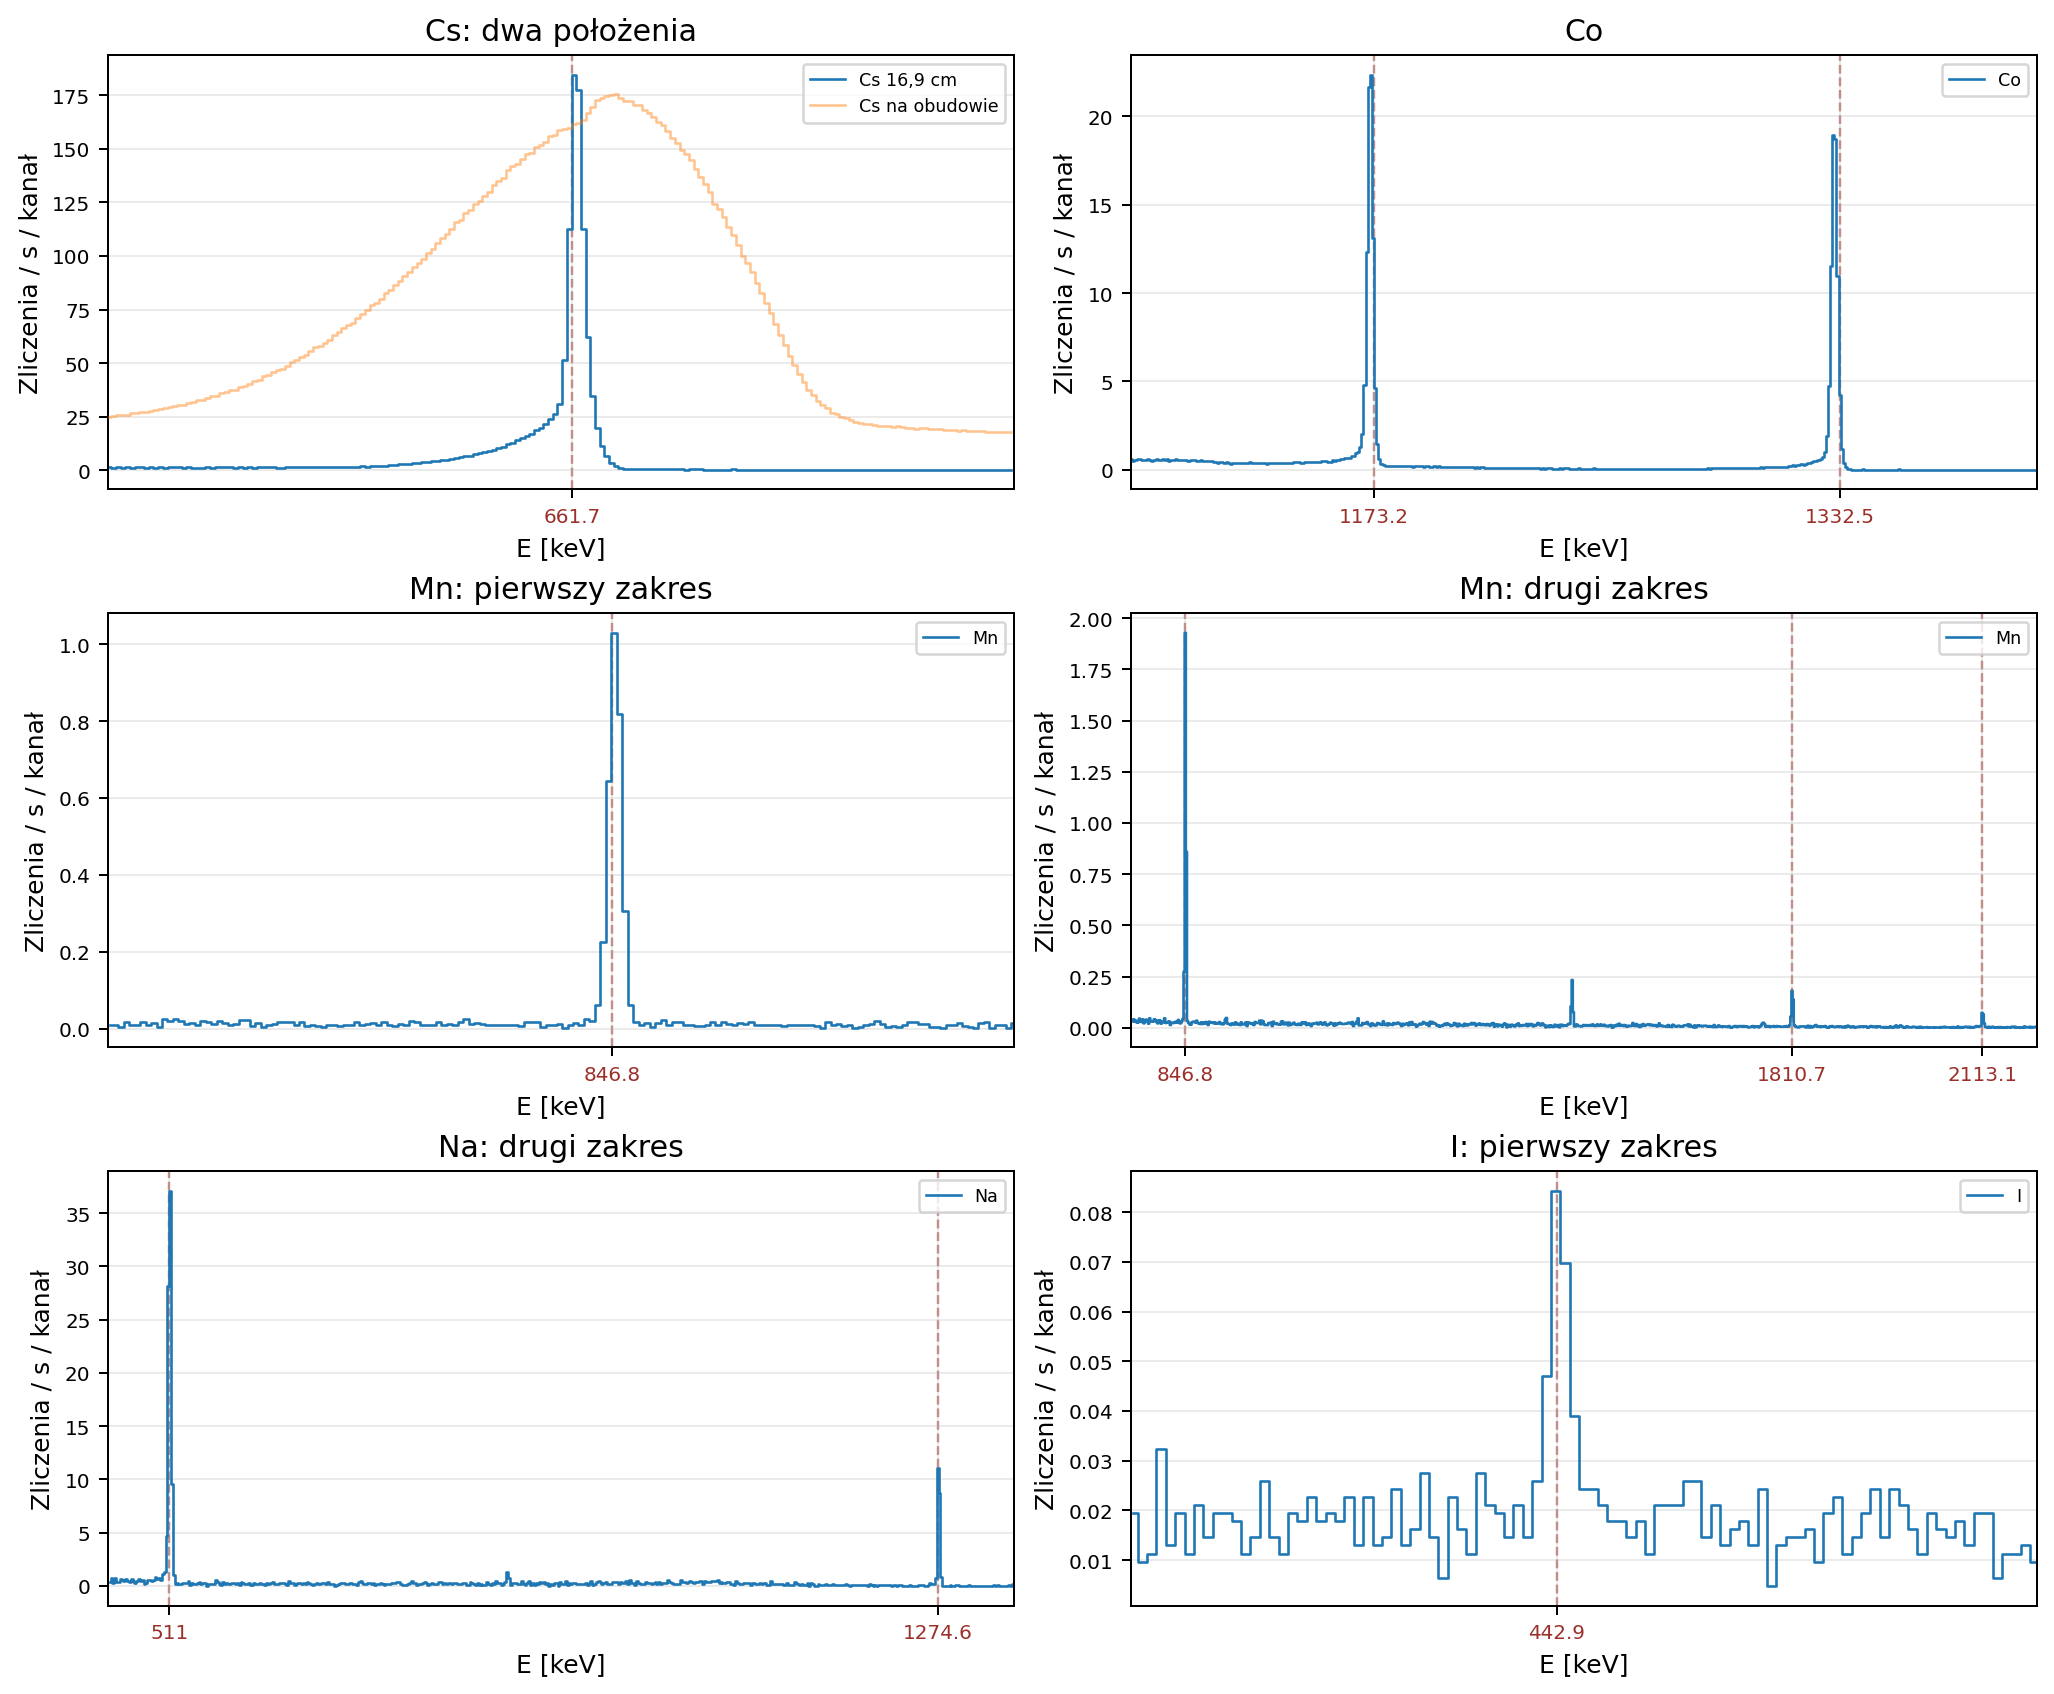
\includegraphics[width=0.9\textwidth]{widma_pomocnicze.png}
\caption{Wybrane widma pomocnicze w częstości zliczeń.
Czerwone wartości na osi i pionowe linie przerywane
wskazują tablicowe energie linii.}
\label{fig:pomocnicze}
\end{figure*}

\section{Opis eksperymentu}
Widma rejestrowano detektorem HPGe ORTEC GMX25P4-70 połączonym
z programem Tukan z wcześniej wprowadzoną kalibracją energii. Pomiary rozpoczęto od umieszczenia źródła $^{137}$Cs w komorze uruchomionego detektora. Zarejestrowano pięć widm przy różnych położeniach
źródła, przy czym pomiary trwały od około 5 do 17 minut czasu
rzeczywistego. Następnie w analogiczny sposób zarejestrowano
trzy widma $^{60}$Co, każde przez około 6--14 minut.
Zmiana odległości pozwalała obserwować położenia linii,
częstość zliczeń oraz wskazywany przez program czas martwy.
W pomiarze Cs ze źródłem położonym na obudowie detektora
czas żywy wyniósł $619~\mathrm{s}$ przy czasie rzeczywistym
$1046~\mathrm{s}$, co odpowiada około $41\%$ czasu martwego.
Widma te służyły również zapoznaniu się z obsługą układu
pomiarowego.

Następnie dla trzech różnych położeń względem detektora zarejestrowano widma źródła $^{152}$Eu.
Dwa pierwsze pomiary trwały około 6 minut, a trzeci
$526~\mathrm{s}$ czasu rzeczywistego
($522~\mathrm{s}$ czasu żywego). Przy trzecim pomiarze
źródło znajdowało się około $16{,}9~\mathrm{cm}$
od powierzchni obudowy detektora.

Przed rozpoczęciem pomiarów próbek aktywowanych
prowadzono rejestrację tła przez około 19 godzin
i 15 minut. Zapis obejmuje $69260~\mathrm{s}$
czasu żywego oraz zliczenia w 2048 kolejnych kanałach.
Następnie ponownie zarejestrowano widmo $^{152}$Eu
przez $520~\mathrm{s}$ i sprawdzono na nim kalibrację
energii programu Tukan.

Z osłony źródła AmBe wyjęto wcześniej napromienioną
monetę i zarejestrowano jej widmo przez około 72 minuty.
W osłonie znajdowały się także próbki Mn i I.
Folie Au i Cu umieszczono symetrycznie przy przeciwnych
końcach walcowego źródła, gdzie pozostawały podczas
pomiarów pozostałych próbek. Pierwsze widmo Mn
rejestrowano przez $500~\mathrm{s}$. Widoczna była
linia około 847~keV, lecz pierwotny zakres energii
nie pozwalał prześledzić linii o wyższych energiach.
Po zmianie zakresu wykonano drugi pomiar Mn przez
$606~\mathrm{s}$ oraz krótki pomiar Na. Na podstawie
linii tych widm przygotowano w programie kalibrację
energii nowego zakresu. Widmo I mierzono
przez $618~\mathrm{s}$ na poprzednim zakresie energii,
a drugą monetę przez $1500~\mathrm{s}$.

Folię Au o masie $0{,}1328~\mathrm{g}$ napromieniano
około $3{,}5~\mathrm{h}$, a folię Cu o masie
$0{,}1479~\mathrm{g}$ około $4~\mathrm{h}$.
Pierwszy pomiar Au rozpoczęto $61~\mathrm{s}$ po
zdjęciu folii ze źródła. Folię umieszczono wtedy
około $16{,}9~\mathrm{cm}$ od obudowy detektora,
tak jak podczas wybranego pomiaru Eu, i rejestrowano
przez $956~\mathrm{s}$ czasu rzeczywistego.
Ponieważ przy tym położeniu nie rozróżniono linii
około 412~keV od tła, folię przeniesiono bezpośrednio
na obudowę. Drugi pomiar rozpoczęto po łącznie
$1084~\mathrm{s}$ od zakończenia napromieniania
i prowadzono przez $1393~\mathrm{s}$. Folię Cu
położono na obudowie po około $60~\mathrm{s}$
przenoszenia ze źródła AmBe do detektora, a jej widmo rejestrowano przez
$1821~\mathrm{s}$. Czasy aktywacji obu folii oraz
chłodzenia Cu były oszacowaniami. W przypadku Cu
nie zanotowano dokładnie chwili odklejenia folii
od źródła, dlatego czas od zakończenia aktywacji
do początku pomiaru jest przybliżony.

\begin{figure*}[t]
\centering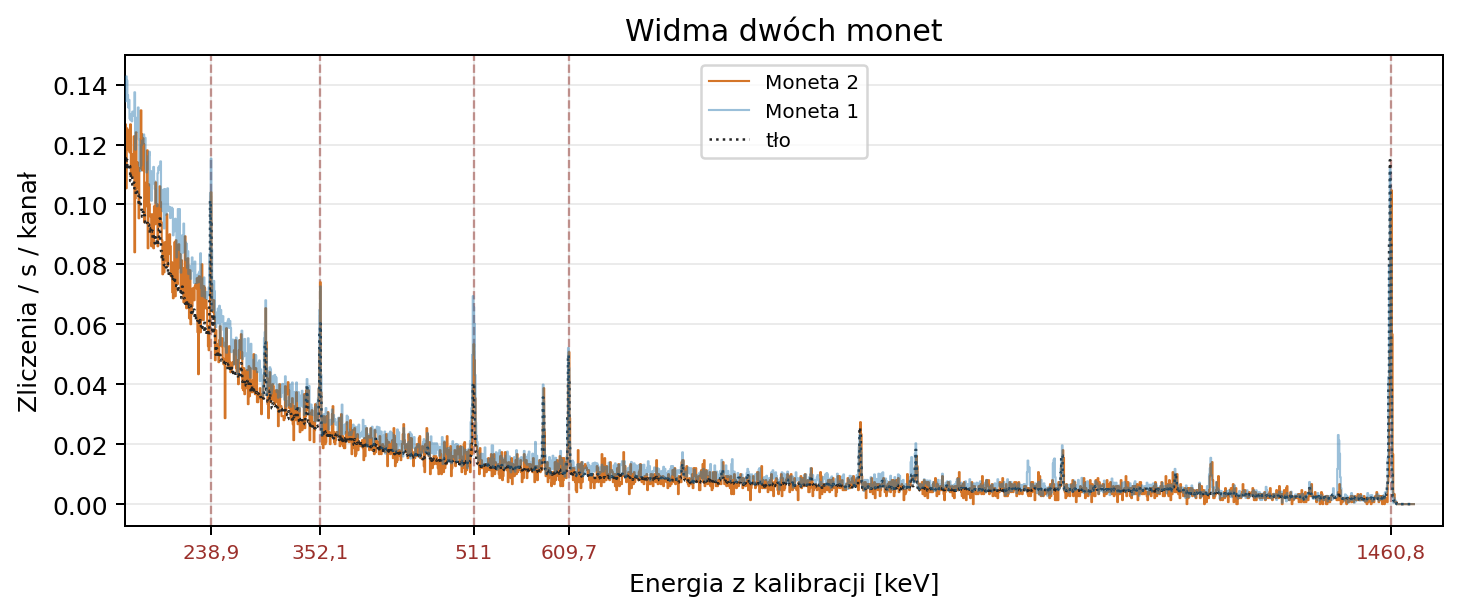
\includegraphics[width=.75\textwidth]{monety.png}
\caption{Widma monet i tło podzielone przez czas żywy.
Wartości na osi i pionowe linie przerywane wskazują
wybrane energie.}
\label{fig:monety}
\end{figure*}




\section{Wyniki i ich dyskusja}
\subsection*{Widma pomocnicze i kalibracja energii}
Energię $E$ rejestrowaną w kanale o numerze $k$ obliczono
z prostej kalibracyjnej $E(k)=ak+b$, gdzie $a$ jest szerokością
kanału w keV, a $b$ przesunięciem skali. Współczynniki dopasowano
do położeń pików znanych linii zapisanych w plikach kalibracji
programu Tukan. Dla pierwszego zakresu, wyznaczonego z linii
$^{152}$Eu, otrzymano
$E(k)=(0{,}72567159k-0{,}56359882)\,\mathrm{keV}$.
W zakresie zmienionym podczas drugiego pomiaru Mn,
wyznaczonym z linii Na i Mn, uzyskano
$E(k)=(1{,}81930247k-1{,}34743419)\,\mathrm{keV}$.

Na rys.~\ref{fig:pomocnicze} zestawiono wybrane widma Cs,
Co, Mn, Na i I. W pomiarze Cs z większej odległości
zaobserwowano wąski pik o maksimum przy
$(662{,}0\pm0{,}2)$~keV. Po umieszczeniu źródła na
obudowie detektora częstość zliczeń wzrosła, lecz
widmo zostało silnie zniekształcone. Szerokie maksimum
wypadło przy $(668{,}5\pm0{,}2)$~keV. Ze względu
na około $41\%$ czasu martwego tej serii nie użyto
do precyzyjnej kontroli kalibracji. W widmie Co
widoczne były dwa maksima przy
$(1172{,}1\pm0{,}2)$ i $(1330{,}3\pm0{,}2)$~keV.

Zmiana zakresu rejestracji była dokonana dla drugiego pomiaru Mn. W pierwszym pomiarze maksimum miało
energię $(847{,}0\pm0{,}2)$~keV. W drugim, po
przeliczeniu kanałów nową kalibracją, otrzymano
$(846{,}4\pm0{,}5)$, $(1810{,}7\pm0{,}5)$
i $(2112{,}7\pm0{,}5)$~keV. W widmie Na
zaobserwowano maksima $(511{,}7\pm0{,}5)$
i $(1274{,}0\pm0{,}5)$~keV, a w I
$(442{,}8\pm0{,}2)$~keV. Podane niepewności
oznaczają wyłącznie odczyt środka kanału
$u_{\rm bin}=\Delta E/\sqrt{12}$, gdzie $\Delta E=a$
jest szerokością kanału danego zakresu.



Widma obu monet porównano po przeliczeniu ilosci zliczeń przez
czasy żywe, co pokazano na rys.~\ref{fig:monety}.
W pierwszym widmie maksimum linii w pobliżu
511~keV wyniosło $(510{,}3\pm0{,}2)$~keV,
a w drugim $(511{,}0\pm0{,}2)$~keV. Także tutaj
niepewność dotyczy jedynie odczytu kanału.
Na wykresie zaznaczono ponadto energie 239, 352,
610 i 1461~keV. Porównano częstości zliczeń netto
w tych liniach z tłem. Linie 239, 352 i 610~keV
pochodzą od naturalnych szeregów promieniotwórczych,
a 1461~keV od $^{40}$K. W obu monetach ich częstości
były zgodne z tłem w granicach niepewności, więc nie
pochodzą z monet. Wyraźnie większą częstość niż
w tle zaobserwowano tylko w linii 511~keV:
$(0{,}262\pm0{,}011)\,\mathrm{s^{-1}}$ dla pierwszej
i $(0{,}152\pm0{,}016)\,\mathrm{s^{-1}}$ dla drugiej
monety, wobec $(0{,}112\pm0{,}002)\,\mathrm{s^{-1}}$
w tle. Częstości te wyznaczono jako zliczenia
w oknie $\pm4~\mathrm{keV}$ wokół linii po odjęciu
kontinuum z sąsiednich kanałów, podzielone przez
czas żywy. Nadwyżka wskazuje na emiter pozytonów
powstały w monecie, najpewniej $^{64}$Cu z aktywacji
miedzi. Pozwala to stwierdzić obecność miedzi
w pierwszej monecie. Dla drugiej nadwyżka wynosi
około $2{,}5$ niepewności, więc jest tylko
przesłanką. Innych linii aktywacyjnych
nie wyróżniono ponad tłem, dlatego na tej podstawie
nie można określić pozostałych składników stopu.

\begin{figure*}[t]
\centering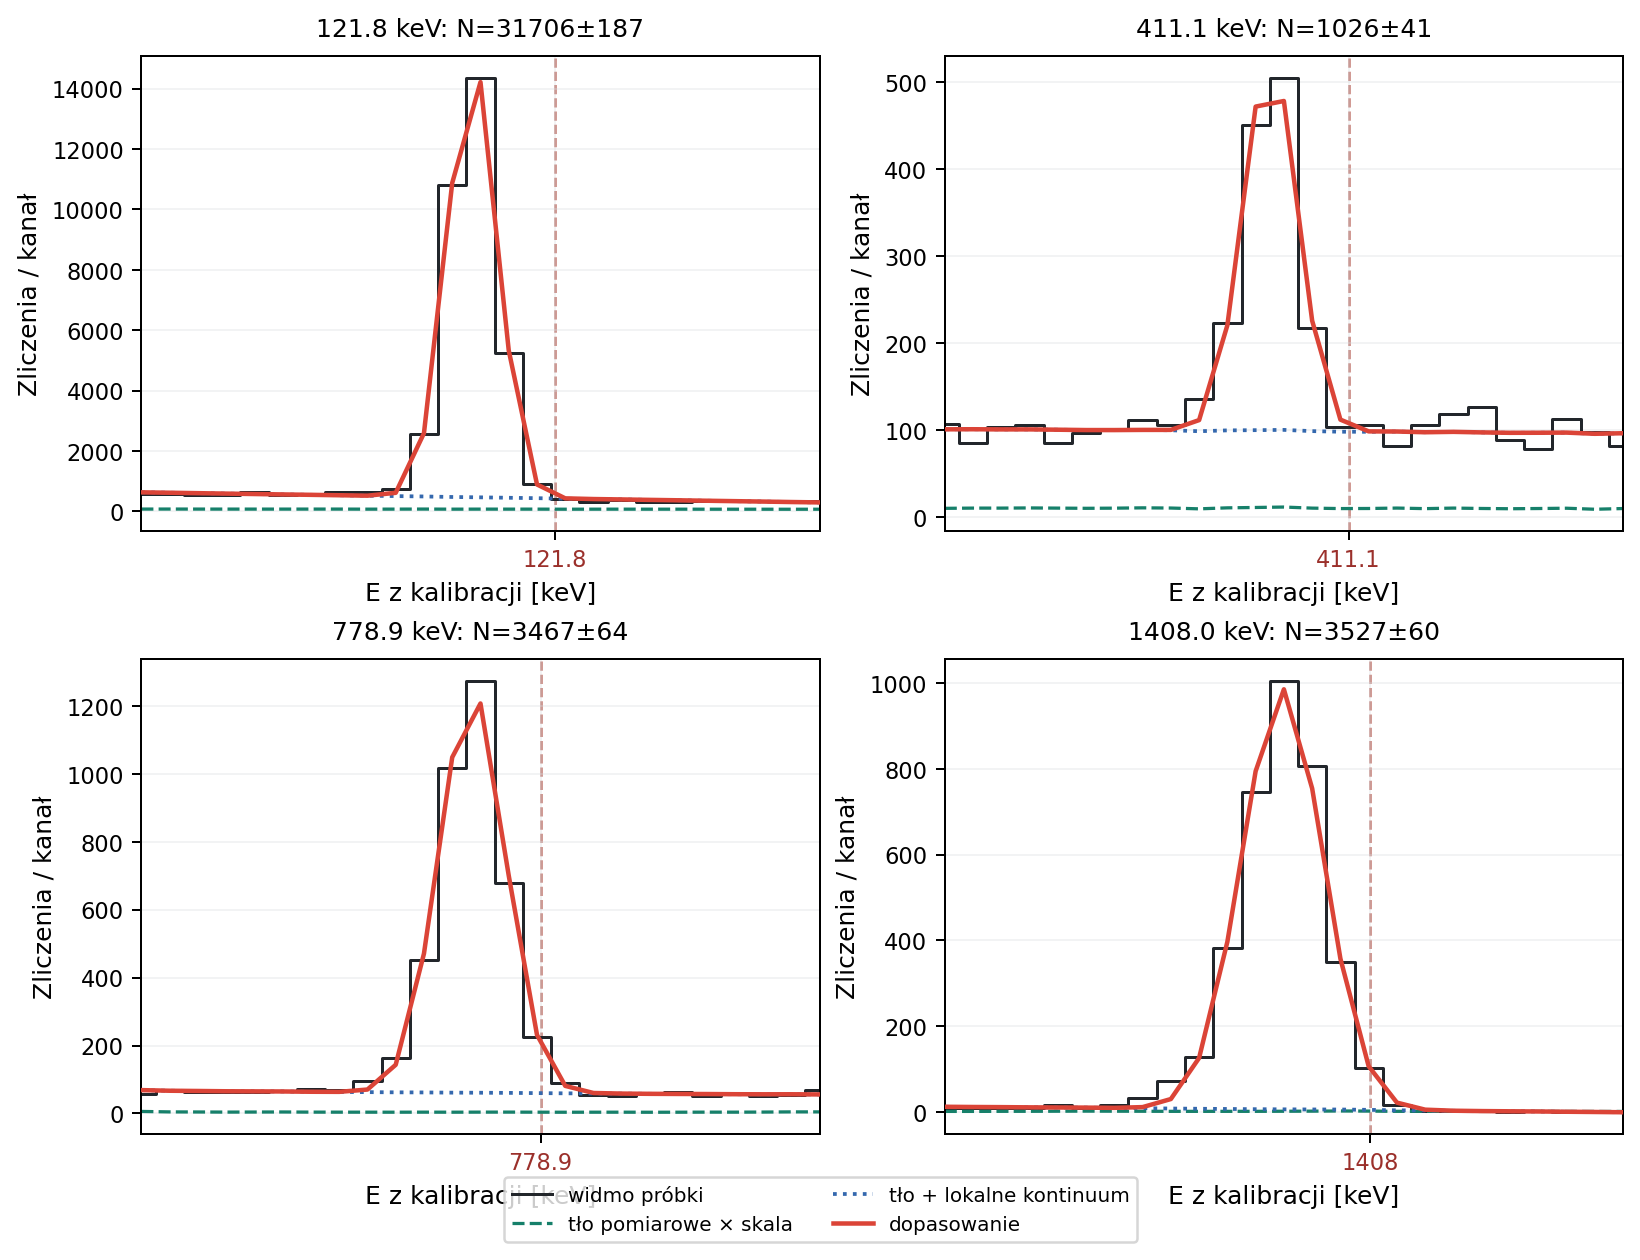
\includegraphics[width=.8\textwidth]{eu_dopasowania.png}
\caption{Wybrane linie $^{152}$Eu. Czarne: widmo; zielone:
przeskalowane tło; niebieskie: tło i kontinuum; czerwone:
dopasowanie. Oś energii wynika z kalibracji wyznaczonej
z linii tego widma, a linie przerywane wskazują energie
ze świadectwa.}
\label{fig:eu_gauss}
\end{figure*}

\subsection*{Pola pików $^{152}$Eu i wydajność}
Do wyznaczenia wydajności wybrano trzeci pomiar Eu
z odległości $16{,}9~\mathrm{cm}$ od powierzchni detektora. Czas martwy wynosił
w nim poniżej $1\%$, a wszystkie linie ze świadectwa
były dobrze rozdzielone. W zapisanej kalibracji
programu środki dopasowanych pików leżały jednak
o $1{,}5$--$2{,}3$~keV poniżej energii ze świadectwa,
podczas gdy dla widma Eu zarejestrowanego przed
pomiarami folii różnica wynosiła około $0{,}2$~keV.
Ponieważ Eu jest źródłem kalibracyjnym, oś energii
tego widma wyznaczono ponownie z położeń 13 linii,
otrzymując
$E(k)=(0{,}725467k+1{,}5159)\,\mathrm{keV}$.
Po tej korekcie odchylenia od energii ze świadectwa
nie przekraczały $0{,}25$~keV, z wyjątkiem linii
1408~keV ($-0{,}58$~keV).

Samo przesunięcie osi nie zmienia pól pików,
ponieważ przedział dopasowania ustawiano na maksimum
w kanałach, a wydajność przypisywano energii ze
świadectwa. Ma ono jednak znaczenie przy odejmowaniu
tła, które zarejestrowano przy nieco innej kalibracji. Dlatego tło przeniesiono na oś
energii widma Eu przez interpolację skumulowanej
liczby zliczeń, a następnie przeskalowano je czynnikiem
$\alpha=t_{l,\rm Eu}/t_{l,\rm tlo}$, gdzie $t_l$ oznacza
czas żywy. Dla każdego piku w lokalnych zakresach wartości energii dopasowano rozkład Gaussa
zintegrowany po szerokości kanału i prostą opisującą kontinuum:
\begin{equation}
\begin{aligned}
n_i^{\rm mod}={}&A\left[
\Phi\!\left(\frac{k_i+\frac12-\mu}{s}\right)\right.\\
&\left.{}-\Phi\!\left(\frac{k_i-\frac12-\mu}{s}\right)
\right]+B+C(k_i-\mu).
\end{aligned}
\label{eq:gauss}
\end{equation}
Tu $n_i^{\rm mod}$ jest przewidywaną liczbą zliczeń
w kanale o numerze $k_i$, $\Phi$ dystrybuantą
standardowego rozkładu normalnego, $\mu$ środkiem piku
w kanałach, $s$ odchyleniem standardowym piku w kanałach,
$A$ pełnym polem gaussowskim, a $B$ i $C$ wyrazem wolnym
i nachyleniem prostej opisującej kontinuum. Pole netto
$N=A$ i jego niepewność standardowa $u(N)$ pochodzą
z dopasowania po odjęciu tła. Ze środka piku obliczono
energię $E_{\rm fit}=a\mu+b$, przyjmując współczynniki
kalibracji danego widma, a z szerokości piku
szerokość połówkową
$\mathrm{FWHM}=2\sqrt{2\ln2}\,a s$. Cztery przykładowe
dopasowania są na rys.~\ref{fig:eu_gauss}.


Aktywność ze świadectwa $A_0=(101{,}3\pm2{,}4)$~kBq
z 1.01.2018 i okres $T_{1/2,\rm Eu}=(13{,}522\pm0{,}016)$~roku
przeliczono na chwilę pomiaru:
\begin{equation}
A_{\rm Eu}=A_0\,2^{-\Delta t/T_{1/2,\rm Eu}}
=(64{,}56\pm1{,}53)\,\mathrm{kBq},
\label{eq:activity}
\end{equation}
gdzie $\Delta t$ oznacza czas od daty wzorcowania do pomiaru. Niepewność $2{,}4$~kBq
warunkowo przyjęto jako standardową; jej rodzaju nie podano
na widocznej stronie świadectwa. Zmiana aktywności w ciągu
$526~\mathrm{s}$ pomiaru była pomijalna.
Wydajność pełnoenergetyczną w geometrii Eu wyznaczono z
\begin{equation}
\varepsilon_{\rm Eu}(E)=
\frac{N_{\rm Eu}(E)}{A_{\rm Eu}I_\gamma(E)t_{l,\rm Eu}},
\label{eq:eff}
\end{equation}
gdzie $N_{\rm Eu}(E)$ jest polem netto linii o energii $E$,
$I_\gamma$ prawdopodobieństwem emisji linii
ze świadectwa~\cite{cert}, a $t_{l,\rm Eu}$ czasem żywym
pomiaru Eu. Wyniki wraz z parametrami dopasowań
zestawiono w tab.~\ref{tab:eu}.
\begin{table*}[t]
\centering\small
\caption{Wszystkie linie $^{152}$Eu dla geometrii
$16{,}9~\mathrm{cm}$: energia ze świadectwa $E$,
prawdopodobieństwo emisji $I_\gamma$, pole netto $N$,
wydajność $\varepsilon$, energia środka dopasowanego
piku $E_{\rm fit}$ i jego szerokość połówkowa FWHM.}
\label{tab:eu}
\begin{tabular}{rrrrrr}
\toprule
$E$ [keV] & $I_\gamma$ [\%] & $N$ & $\varepsilon$ [\%] &
$E_{\rm fit}$ [keV] & FWHM [keV]\\
\midrule
121,8 & 28,4 & $31710\pm190$ & $0,3313\pm0,0081$ & 121,73 & 1,40\\
244,7 & 7,6 & $5457\pm84$ & $0,2131\pm0,0061$ & 244,64 & 1,51\\
344,3 & 26,6 & $14540\pm130$ & $0,1622\pm0,0041$ & 344,24 & 1,58\\
411,1 & 2,4 & $1028\pm42$ & $0,1271\pm0,0060$ & 411,05 & 1,54\\
444,0 & 3,1 & $1435\pm46$ & $0,1374\pm0,0055$ & 443,96 & 1,59\\
778,9 & 13,0 & $3466\pm64$ & $0,0791\pm0,0024$ & 779,00 & 1,93\\
867,4 & 4,2 & $1017\pm40$ & $0,0719\pm0,0033$ & 867,50 & 2,08\\
964,1 & 14,5 & $3196\pm60$ & $0,0654\pm0,0020$ & 964,21 & 2,05\\
1085,8 & 10,1 & $2119\pm50$ & $0,0622\pm0,0021$ & 1086,04 & 2,06\\
1112,1 & 13,4 & $2763\pm56$ & $0,0612\pm0,0019$ & 1112,20 & 2,16\\
1212,9 & 1,4 & $257\pm21$ & $0,0544\pm0,0046$ & 1213,05 & 2,33\\
1299,1 & 1,6 & $269\pm19$ & $0,0499\pm0,0037$ & 1299,16 & 2,10\\
1408,0 & 20,9 & $3527\pm61$ & $0,0501\pm0,0015$ & 1407,42 & 2,46\\
\bottomrule
\end{tabular}
\end{table*}

Punkty dopasowano do funkcji z instrukcji Z40:
\begin{equation}
\ln\varepsilon_{\rm Eu}(E)=c_3x^3+c_2x^2+c_1x+c_0,\quad
x=\ln\!\left(\frac{E}{\mathrm{keV}}\right).
\label{eq:curve}
\end{equation}
Otrzymano bezwymiarowe
$c_3=0{,}067\pm0{,}017$,
$c_2=-1{,}26\pm0{,}29$,
$c_1=7{,}0\pm1{,}7$ i $c_0=-17{,}7\pm3{,}3$.
Podano warunkowe niepewności parametrów z dopasowania,
a obliczenia prowadzono z pełną precyzją współczynników.
Wykres~\ref{fig:efficiency} przedstawia wszystkie 13
punktów i otrzymaną krzywą. Wydajność zmalała
z około $0{,}33\%$ przy 121,8~keV do około
$0{,}05\%$ przy 1408~keV.

\begin{figure*}[t]
\centering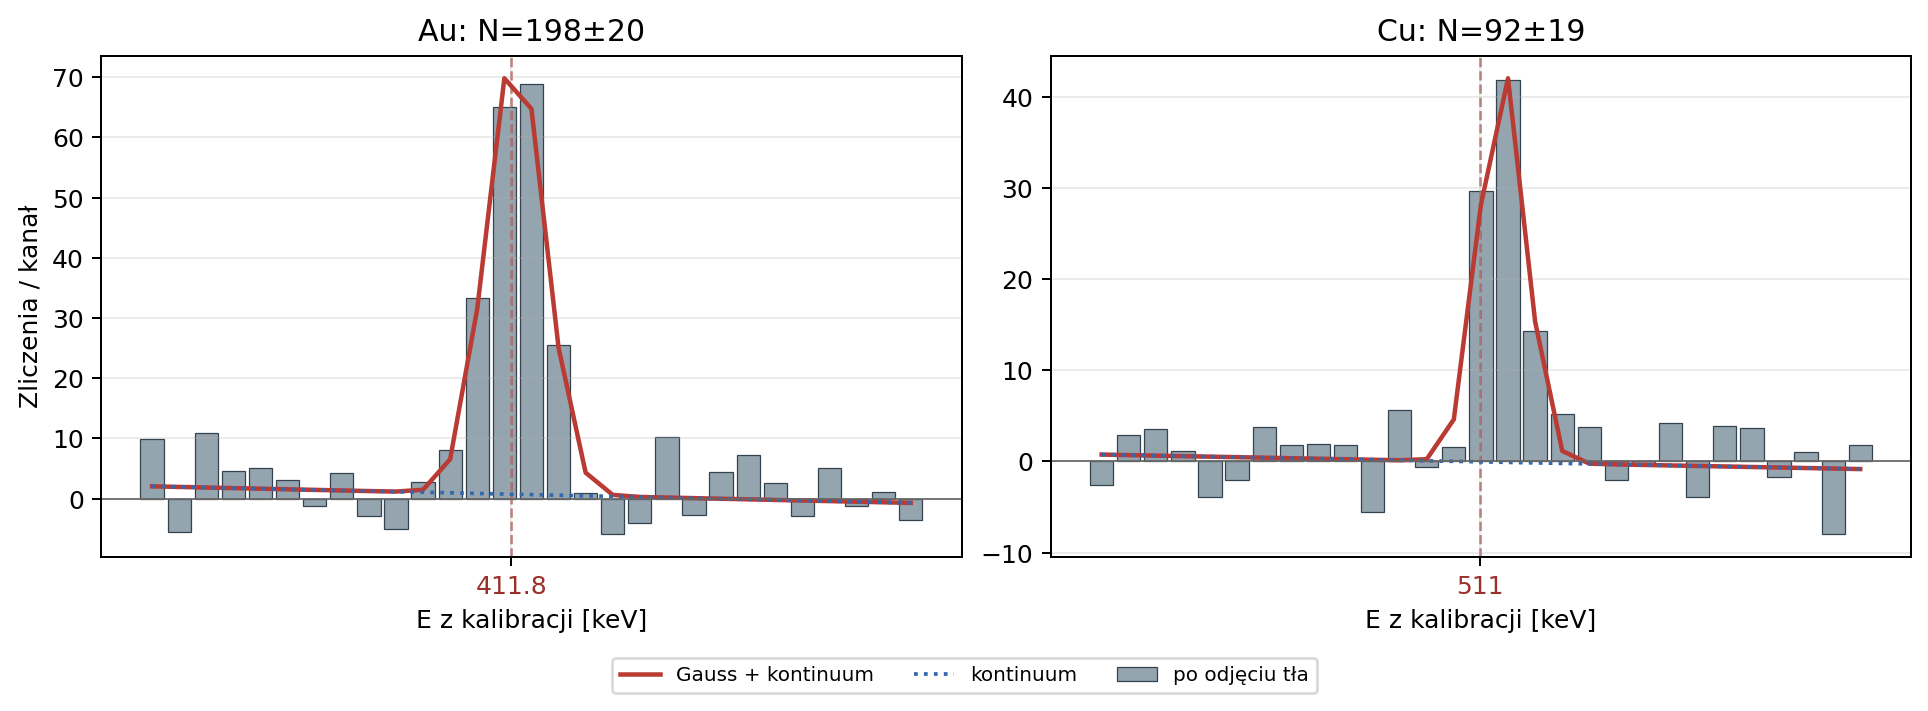
\includegraphics[width=.85\textwidth]{folie_dopasowania.png}
\caption{Lokalne obszary widm Au i Cu po odjęciu
przeskalowanego tła. Słupki oznaczają kanały, linia
czerwona dopasowanie Gaussa z prostą, a niebieska
kropkowana lokalne kontinuum. Pionowe linie
przerywane wskazują energie tablicowe.}
\label{fig:foils}
\end{figure*}
\begin{figure}[t]
\centering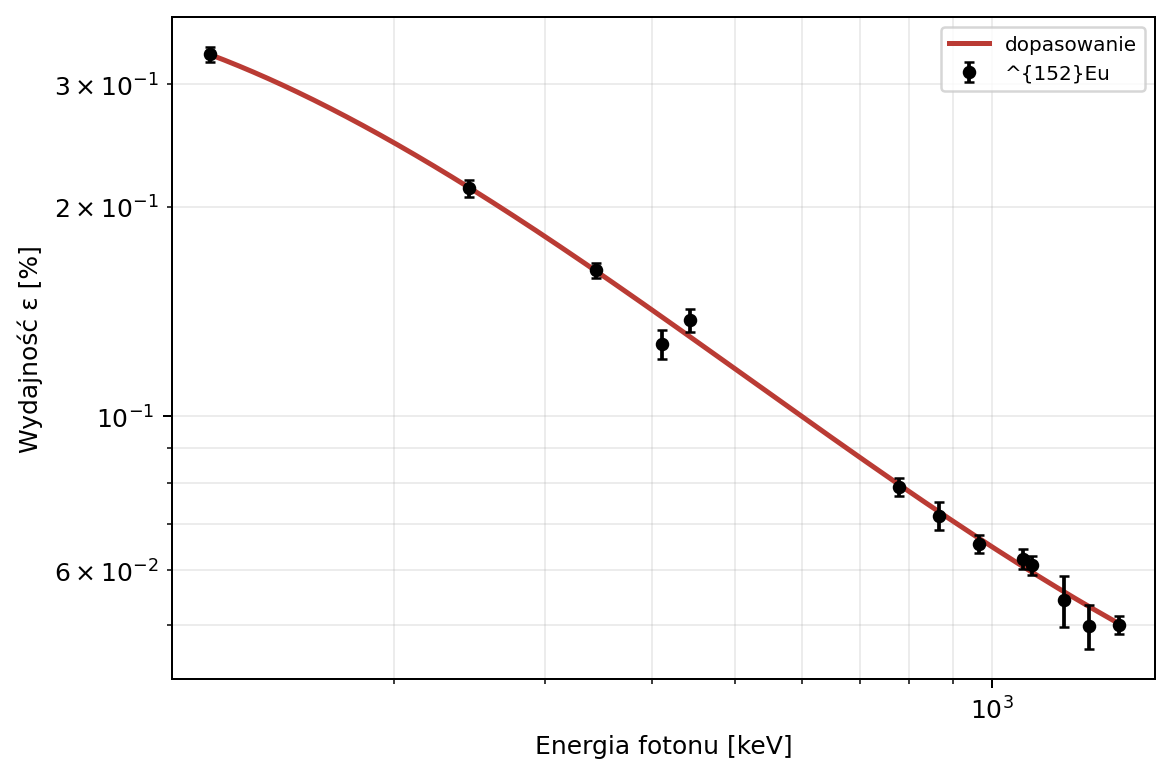
\includegraphics[width=.8\columnwidth]{wydajnosc_eu.png}
\caption{Wydajność pełnoenergetyczna dla trzeciego
pomiaru $^{152}$Eu; dopasowanie pochodzi z równania~(\ref{eq:curve}).}
\label{fig:efficiency}
\end{figure}
\vspace{-2.5mm}

\subsection*{Folie i lokalna gęstość strumienia}
W pierwszym pomiarze Au z odległości $16{,}9~\mathrm{cm}$
pik około 412~keV nie był rozróżnialny od tła.
Po umieszczeniu Au na obudowie dla linii
$411{,}8~\mathrm{keV}$ otrzymano
$N_{\rm Au}=(198{,}5\pm20{,}1)$ zliczeń netto
przy $E_{\rm fit}=(411{,}93\pm0{,}08)$~keV
i $\mathrm{FWHM}=1{,}72$~keV.
W Cu dla obszaru 511~keV uzyskano
$N_{\rm Cu}=(92{,}0\pm19{,}5)$ zliczeń
przy $E_{\rm fit}=(511{,}14\pm0{,}10)$~keV
i $\mathrm{FWHM}=2{,}56$~keV. Linia anihilacyjna
jest szersza od linii gamma o podobnej energii,
co jest oczekiwane ze względu na ruch pary
elektron--pozyton w chwili anihilacji.
Oba dopasowania przedstawiono na rys.~\ref{fig:foils}.
Zgodnie z instrukcją linię 511~keV przypisano reakcji
$^{63}$Cu$(n,\gamma){}^{64}$Cu~\cite{dodatkowe}.


Karta detektora podaje odstęp okno--kryształ
$3~\mathrm{mm}$ oraz długość kryształu
$70~\mathrm{mm}$~\cite{detector}. Przyjęto umowną
płaszczyznę rejestracji w połowie kryształu,
czyli $d_0=0{,}3+7{,}0/2=3{,}8$~cm od obudowy.
Prosty transfer wydajności do geometrii folii
miał postać
\begin{equation}
\begin{aligned}
G&=\left(\frac{16{,}9\,\mathrm{cm}+d_0}{d_0}\right)^2
=29{,}674,\\
\varepsilon_{\rm f}(E)&=G\varepsilon_{\rm Eu}(E).
\end{aligned}
\label{eq:geometry}
\end{equation}
gdzie $G$ jest stosunkiem kwadratów odległości źródła Eu dla której wykonano kalibrację energetyczną, i folii od płaszczyzny rejestracji, a $\varepsilon_{\rm f}$
oszacowaną wydajnością pełnoenergetyczną dla folii na obudowie.
Otrzymano $\varepsilon_{\rm f}(411{,}8\,\mathrm{keV})
=0{,}04120$ dla Au i $\varepsilon_{\rm f}
(511\,\mathrm{keV})=0{,}03410$ dla Cu.

Liczba jąder docelowych wynosi $N_p=mgN_A/M$,
gdzie $m$ oznacza masę, $g$ abundancję izotopu,
$N_A$ stałą Avogadra, a $M$ masę molową.
Dla lokalnej gęstości strumienia $\phi$, przekroju
czynnego $\sigma$ i $\lambda=\ln2/T_{1/2}$ model
aktywacji daje
\begin{align}
N_\gamma={}&\frac{t_l}{t_r}\varepsilon_{\rm f}I_\gamma
\frac{\sigma\phi mgN_A}{M\lambda}
(1-e^{-\lambda t_a})e^{-\lambda t_c}
(1-e^{-\lambda t_r}),\label{eq:counts}\\
\phi={}&\frac{N_\gamma M\lambda t_r e^{\lambda t_c}}
{\varepsilon_{\rm f}I_\gamma t_l\sigma mgN_A
(1-e^{-\lambda t_a})(1-e^{-\lambda t_r})}.
\label{eq:flux}
\end{align}
Tu $N_\gamma$ jest polem netto piku folii ($N_{\rm Au}$
lub $N_{\rm Cu}$), $I_\gamma$ prawdopodobieństwem emisji
analizowanej linii na rozpad, $t_a$ czasem aktywacji,
$t_c$ chłodzenia, $t_l$ pomiaru żywego, a $t_r$ pomiaru
rzeczywistego.
Przeliczono $1\,\mathrm b=10^{-24}\,\mathrm{cm^2}$.
Dla $^{197}$Au$(n,\gamma){}^{198}$Au przyjęto
$\sigma=98{,}8$~b, $T_{1/2}=232675{,}2$~s,
$g=1$, $I_\gamma=0{,}95$, $M=196{,}967$~g/mol.
Dla $^{63}$Cu$(n,\gamma){}^{64}$Cu:
$\sigma=4{,}5$~b, $T_{1/2}=46080$~s,
$g=0{,}6915$, $I_\gamma=0{,}38$ (fotony 511~keV na rozpad),
$M=62{,}93$~g/mol~\cite{dodatkowe}.
Rzeczywiste i żywe czasy pomiaru wyniosły odpowiednio
$(1393,1392)$~s dla Au i $(1821,1819)$~s dla Cu.
Po podstawieniu do równania~(\ref{eq:flux}) otrzymano
\begin{align}
\phi_{\rm Au}&=(2480\pm280)\,\mathrm{n\,cm^{-2}s^{-1}},\\
\phi_{\rm Cu}&=(4620\pm1000)\,\mathrm{n\,cm^{-2}s^{-1}}.
\label{eq:results}
\end{align}
Porównując wartość bezwzględną różnicy obu wyników
z $\kappa$-krotnością sumy ich niepewności, otrzymujemy
\begin{equation}
\begin{aligned}
\left\lvert\phi_{\rm Cu}-\phi_{\rm Au}\right\rvert
&=\lvert4620-2480\rvert=2140\\
&<\kappa\cdot(1000+280)=\kappa\cdot1280.
\end{aligned}
\label{eq:zgodnosc}
\end{equation}
Warunek jest spełniony dopiero dla $\kappa=2$,
a wynik z Cu jest około $1{,}86$ razy większy.

Na podstawie otrzymanych strumieni oszacowano także
całkowitą emisję neutronów źródła $Q$. Z masy i grubości
folii, $0{,}002$~cala ($50{,}8~\mu$m) dla Au
i $0{,}005$~cala ($127~\mu$m) dla Cu, przy gęstościach
tablicowych wynika, że są to krążki o promieniu
$R_{\rm Au}=6{,}56$~mm i $R_{\rm Cu}=6{,}43$~mm.
Folie przyklejono do podstaw kapsuły źródła o wysokości
$H=19{,}2$~mm~\cite{z40}. Traktując źródło jako punktowe
i izotropowe, położone w środku kapsuły, skorzystano
z zależności
\begin{equation}
\phi=Q\left\langle\frac{1}{4\pi r^2}\right\rangle,
\label{eq:Q}
\end{equation}
gdzie $r$ jest odległością od środka kapsuły do punktu
folii, a średnią $\langle\cdot\rangle$ obliczono po
powierzchni folii. Wymiary geometryczne przyjęto jako
dokładne, dlatego niepewność względna $Q$ jest równa
niepewności względnej $\phi$. Otrzymano
\begin{align}
Q_{\rm Au}&=(3{,}50\pm0{,}39)\cdot10^4~\mathrm{n/s},\\
Q_{\rm Cu}&=(6{,}5\pm1{,}4)\cdot10^4~\mathrm{n/s}.
\label{eq:Qresults}
\end{align}
Wysokość $19{,}7$~mm z rysunku w instrukcji
zwiększa obie wartości o około $4\%$.
Porównując je z emisją podaną w instrukcji
$Q_{\rm ref}=(7{,}7\pm1{,}5)\cdot10^5~\mathrm{n/s}$~\cite{z40}
analogicznie do równania~(\ref{eq:zgodnosc}), warunek
zgodności wymagałby $\kappa>4{,}8$ dla Au i $\kappa>4{,}3$
dla Cu. Otrzymane wartości są około
12--22 razy mniejsze od $Q_{\rm ref}$ i nie są
z nią zgodne. Folie z przekrojami termicznymi
rejestrują bowiem głównie neutrony spowolnione
w parafinie, a nie pierwotne neutrony prędkie,
dla których prawo $1/r^2$ byłoby słuszne.

Różnicę między wynikami z Au i Cu można wyjaśnić kilkoma czynnikami.
Przeliczenie wydajności prawem odwrotnych kwadratów
z nieznanym $d_0$ jest w tak bliskiej geometrii tylko
przybliżeniem, ale ten sam współczynnik $G$ wchodzi
do obu wyników, więc słabo tłumaczy różnicę między nimi.

W pomiarze Cu dodatkową trudność sprawiała silna
linia 511~keV obecna w tle. Po jej odjęciu pozostał
pik z niepewnością względną około $21\%$. Założono
również, że cały ten pik pochodzi z rozpadu
$^{64}$Cu, chociaż fotony anihilacyjne o tej energii
mogą pochodzić także z innych źródeł. Dodatkowe
zliczenia zawyżałyby wynik z Cu, co jest zgodne
z kierunkiem obserwowanej różnicy.

Ogólnie, na oba wyniki mogły wpływać czynniki
związane z samą aktywacją. Czasy napromieniania
folii były jedynie szacowane. Zmiana $t_a$
o $\pm0{,}5$~h zmienia wynik Au o $-12$ do $+16\%$,
a Cu o $-10$ do $+13\%$. Folie były też przenoszone
od źródła do detektora, a dla Cu czas od odklejenia
folii do początku pomiaru oszacowano tylko
w przybliżeniu. Przy czasie połowicznego zaniku
$^{64}$Cu wynoszącym około $12{,}8$~h skrócenie
$t_c$ o połowę zmienia jednak wynik Cu
o mniej niż $0{,}1\%$. Folie znajdowały się po przeciwnych
stronach walcowego źródła, więc strumień neutronów
w ich miejscu mógł się różnić. Użyte przekroje
czynne są wartościami dla neutronów termicznych
i nie opisują całego widma energii neutronów
źródła AmBe. Tych efektów nie uwzględniono
w podanych niepewnościach.

Dokładność można by poprawić, mierząc wydajność
detektora w tej samej geometrii co folie, czyli
umieszczając źródło Eu bezpośrednio na obudowie.
Należałoby również dokładnie zapisywać chwile
umieszczenia i wyjęcia folii z osłony źródła oraz
wydłużyć pomiar Cu, aby zmniejszyć niepewność pola
piku 511~keV.

\section{Podsumowanie i wnioski}
Zarejestrowane widma Cs, Co, Mn, Na i I pozwoliły
sprawdzić położenia linii w obu zakresach rejestracji.
Przy czasie martwym około $41\%$ widmo Cs ulegało
wyraźnemu zniekształceniu.

Na podstawie 13 linii $^{152}$Eu wyznaczono
zależność wydajności pełnoenergetycznej detektora
od energii w geometrii $16{,}9~\mathrm{cm}$.
Wydajność malała z około $0{,}33\%$ przy 121,8~keV
do około $0{,}05\%$ przy 1408~keV. Korekta osi
energii widma Eu o około 2~keV nie zmieniła
w istotny sposób pól pików ani wydajności.

Pierwszy pomiar Au z większej odległości nie
ujawnił piku 412~keV ponad tłem, dlatego do obliczeń
wykorzystano pomiar folii na obudowie. Lokalna
gęstość strumienia neutronów wyznaczona z folii
złotej wyniosła $(2480\pm280)\,\mathrm{n\,cm^{-2}s^{-1}}$,
a z folii miedzianej
$(4620\pm1000)\,\mathrm{n\,cm^{-2}s^{-1}}$.
Wyniki są zgodne dopiero w granicach podwójnej
sumy niepewności. Za bardziej wiarygodny można
uznać wynik z Au, ponieważ linia 412~keV jest
charakterystyczna dla $^{198}$Au, a jej pole
wyznaczono z mniejszą niepewnością względną.
Oba wyniki należy traktować jako oszacowania.
Zastosowany model jest mocno przybliżony:
przeliczenie wydajności prawem odwrotnych
kwadratów w geometrii kontaktowej, termiczne
przekroje czynne oraz szacowane czasy aktywacji,
przenoszenia i chłodzenia folii, szczególnie Cu,
wnoszą błędy systematyczne porównywalne z podanymi
niepewnościami lub większe. Oszacowana z nich
emisja źródła, $(3{,}50\pm0{,}39)\cdot10^4$
i $(6{,}5\pm1{,}4)\cdot10^4~\mathrm{n/s}$, jest
12--22 razy mniejsza od wartości z instrukcji,
więc lokalnego strumienia neutronów termicznych
nie można bezpośrednio przeliczyć na emisję
źródła AmBe.

Widma monet wykazały nadwyżkę linii 511~keV nad tłem,
co wskazuje na miedź co najmniej w pierwszej monecie.

{\small\begin{thebibliography}{9}
\bibitem{z40} Instrukcja do ćwiczenia Z40,
\emph{Aktywacja neutronowa}, II Pracownia Fizyczna, UJ, s.~1--7.
\bibitem{dodatkowe} \emph{Aktywacja neutronowa — materiały
dodatkowe}, tabela parametrów reakcji Au i Cu.
\bibitem{cert} Świadectwo wzorcowania źródła
$^{152}$Eu nr BW/Z-62/154/17, 5.12.2017, s.~2.
\bibitem{detector} ORTEC, \emph{GMX Series HPGe Coaxial
Detector System}, karta modelu GMX25P4-70, załącznik 2.
\end{thebibliography}}

\appendix
\section{Rachunek niepewności}
Niepewność $u(N)$ pola netto pochodzi z lokalnego
dopasowania równania~(\ref{eq:gauss}) po odjęciu tła.
Z prawa przenoszenia dla
równania~(\ref{eq:activity}) otrzymano
\begin{equation}
u(A)=A\sqrt{\left(\frac{u(A_0)}{A_0}\right)^2+
\left(\frac{\ln2\,\Delta t}{T_{1/2,\rm Eu}^2}
u(T_{1/2,\rm Eu})\right)^2}.
\label{eq:uactivity}
\end{equation}
Przy niezależnych $N$ i $A$ zastosowano
\begin{align}
u(\varepsilon)&=\varepsilon\sqrt{
\left(\frac{u(N)}{N}\right)^2+
\left(\frac{u(A)}{A}\right)^2},\label{eq:ueff}\\
u(\phi)&=\phi\sqrt{
\left(\frac{u(N_\gamma)}{N_\gamma}\right)^2+
\left(\frac{u(\varepsilon_{\rm Eu})}
{\varepsilon_{\rm Eu}}\right)^2}.
\label{eq:uflux}
\end{align}
$I_\gamma$, czasy żywe, masy, wymiary folii, $G$
i parametry tablicowe przyjęto jako dokładne (brak
podanych niepewności), a $u(\varepsilon_{\rm Eu})$
przy energii folii oszacowano z najbliższego punktu Eu i $u(A)$.
\end{document}
